\documentclass[11pt]{article}
    \usepackage{amsmath}
    \usepackage[pdftex]{graphicx}
    %\usepackage[usenames,dvipsnames,svgnames,table]{xcolor}
    \usepackage{amsmath,amsthm,amssymb,color,wrapfig,floatflt,amsfonts,listings,fancyhdr}
    \usepackage[parfill]{parskip}
    %\pagestyle{plain}
    \setlength\topmargin{.1cm}
    %\setlength\textheight{8in}
    \setlength\oddsidemargin{.1in}
    \setlength\evensidemargin{.1in}
    \setlength\textwidth{6.51in}
    %\setlength\headheight{52.5pt}
    \usepackage{fancyhdr}
    \usepackage[algosection, boxruled, linesnumbered]{algorithm2e}
    \pagestyle{fancy}
    \lhead{Arvind Ramaswami}
    \rhead{HW1}
    \chead{CS 4641 Machine Learning}
    \lfoot{}
    \cfoot{Page {\thepage}}
    \rfoot{}
    \newcommand{\RR}{\mathbb{R}}
    \newcommand{\CC}{\mathbb{C}}
    \newcommand{\HH}{\mathbb{H}}
    \newcommand{\BB}{\mathbb{B}}
    \newcommand{\ZZ}{\mathbb{Z}}
    \newcommand{\QQ}{\mathbb{Q}}
    \newcommand{\NN}{\mathbb{N}}
    \newcommand{\cP}{\mathcal{P}}
    \renewcommand{\And}{\wedge}
    \newcommand{\Or}{\vee}
    \newcommand{\Implies}{\Rightarrow}
    \newcommand{\Not}{\sim}
    \begin{document}
        \section{Classification problems}
            \subsection{Pima Indians Diabetes Dataset}

            This classification problem involves predicting whether or not a person has diabetes
            based on certain features.

            The features are: Pregnancies, Glucose, BloodPressure, SkinThickness, Insulin, BMI, DiabetesPedigreeFunction, Age.

            The dataset has 768 entries.

            This classification problem is interesting since it is not necessary
            clear whether someone has diabetes given those limited features, so there
            is not necessarily a clearly separable boundary. Running different algorithms
            in this problem should give some insight on how to find a proper boundary for
            such a dataset.

            \subsection{Predicting whether mushrooms are edible}

            The objective of this classification problem is to predict
            whether or not a mushroom is edible or poisonous, based on a set
            of given features.

            The features are: cap-shape, cap-surface, cap-color, bruises, odor, gill-attachment, gill-spacing, gill-size, gill-color, stalk-shape, stalk-root, stalk-surface-above-ring, stalk-surface-below-ring, stalk-color-above-ring, stalk-color-below-ring, veil-type, veil-color, ring-number, ring-type, spore-print-color, population, habitat

            The dataset contains 8,124 data points in total.


        
        \section{Results}

        \subsection{Decision Trees}
        The pruning used for the decision trees was caused by setting a limit on the maximum depth.

        Here are the plots:

        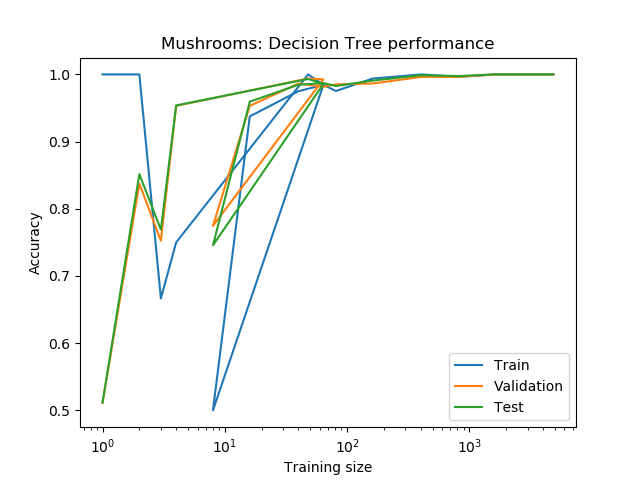
\includegraphics[width=8cm]{mushrooms/mushroom_dt_trainingsize.png}
        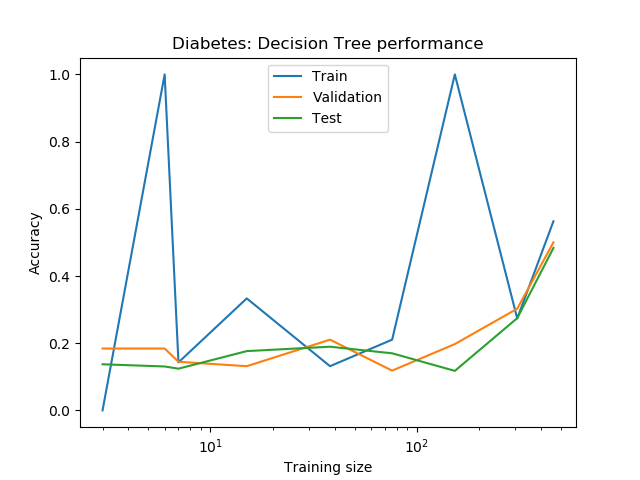
\includegraphics[width=8cm]{diabetes/diabetes_dt_trainingsize.png}

        \subsection{Neural Networks}

        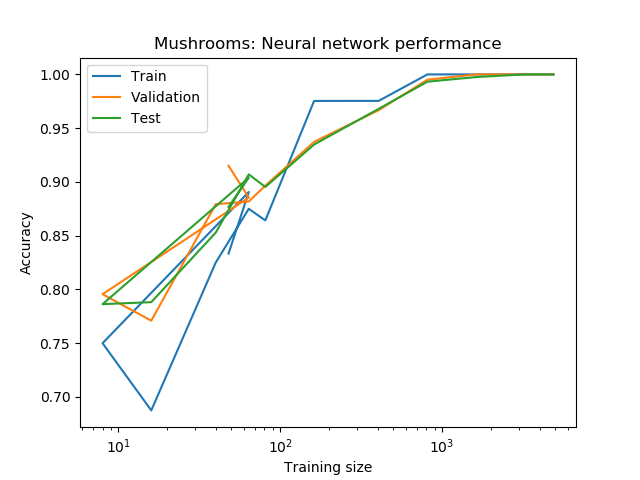
\includegraphics[width=8cm]{mushrooms/mushroom_nn_trainingsize.png}
        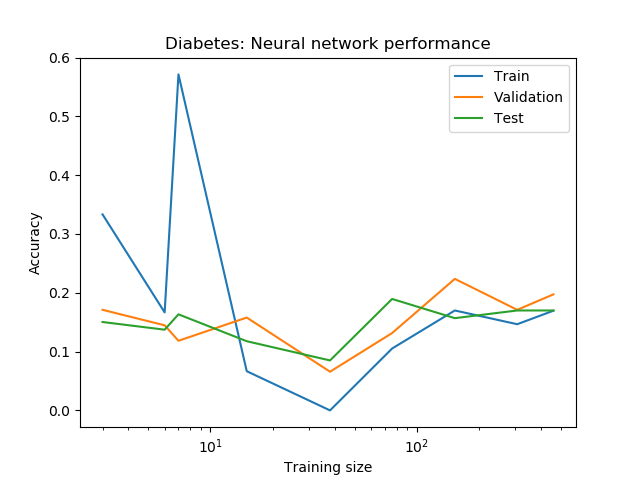
\includegraphics[width=8cm]{diabetes/diabetes_nn_trainingsize.png}

        \subsection{Boosting}
        The experiments in this project used an AdaBoost classifier with a base estimator of decision trees.
        The max depth of the decision trees (for sake of pruning) and the number of trees (base estimators)
        in the boosted classifier were varied.

        Here are the plots taken for boosting:
        
        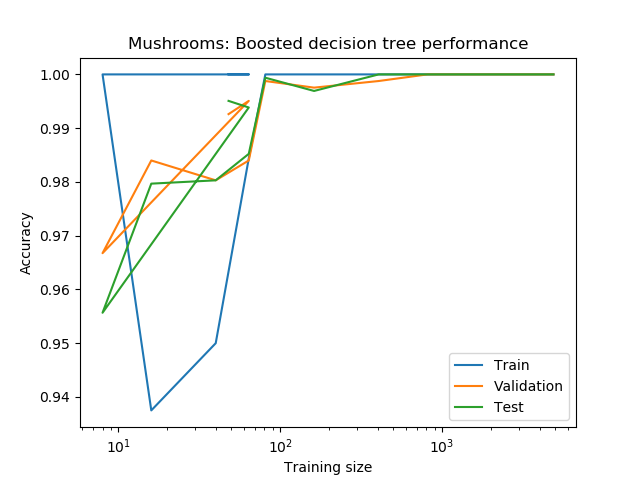
\includegraphics[width=8cm]{mushrooms/mushroom_boost_trainingsize.png}
        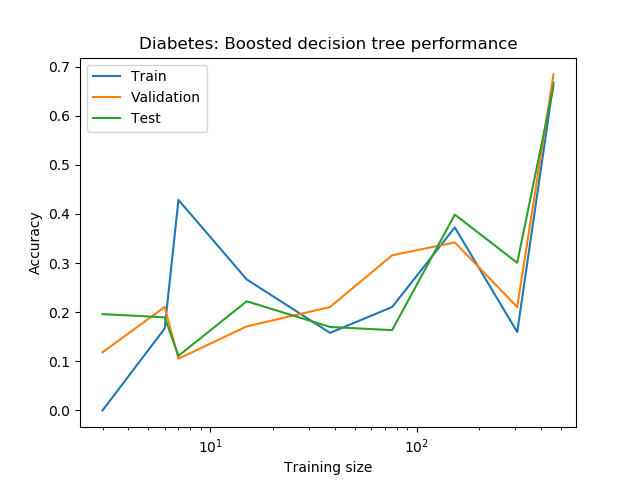
\includegraphics[width=8cm]{diabetes/diabetes_boost_trainingsize.png}

        \subsection{Support Vector Machines}
        The Support Vector Machines were tested with the linear kernel function and the RBF kernel function.

        The SVM plots are shown below:

        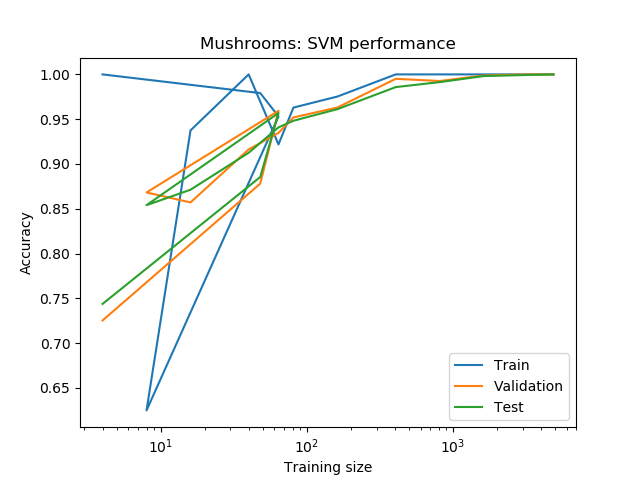
\includegraphics[width=8cm]{mushrooms/mushroom_svm_trainingsize.png}
        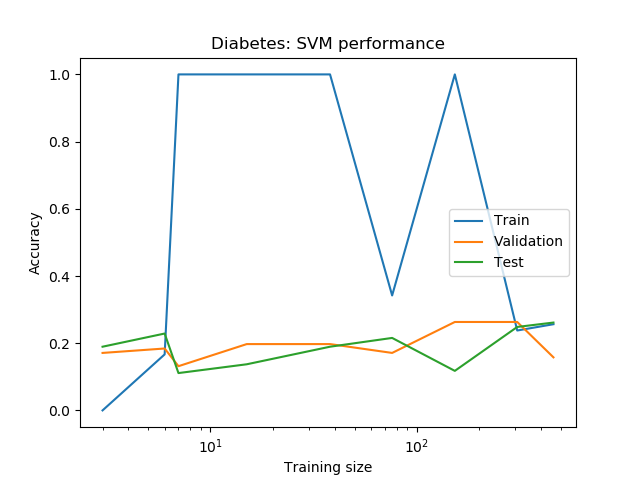
\includegraphics[width=8cm]{diabetes/diabetes_svm_trainingsize.png}

        \subsection{k-Nearest Neighbors}
        The KNN classifiers were tested with varying K values.

        Here are the KNN plots:

        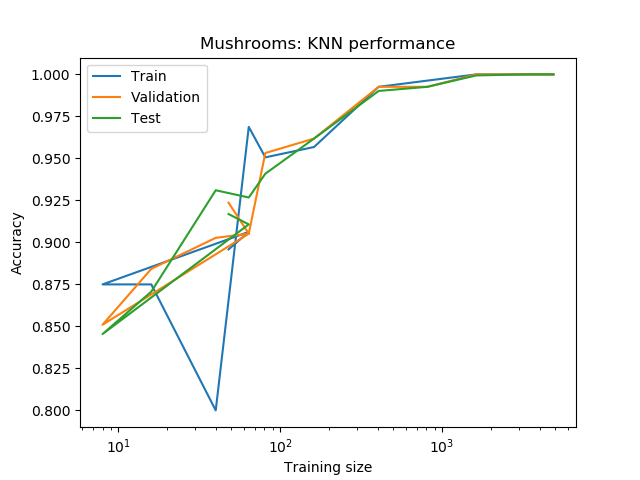
\includegraphics[width=8cm]{mushrooms/mushroom_knn_trainingsize.png}
        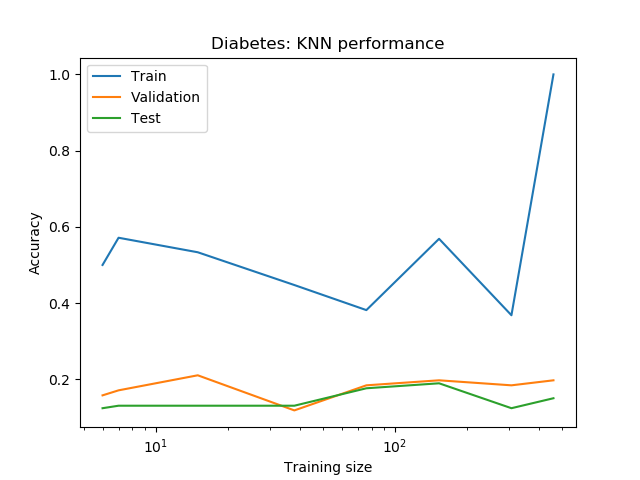
\includegraphics[width=8cm]{diabetes/diabetes_knn_trainingsize.png}

        \section{Analysis}

        \subsection{Decision Trees}


        Decision trees are very effective at learning the mushroom data even with a relatively
        small training size of 100 examples. This is because the values of the inputs
        are discretized, so there is a relatively small number of input combinations (a few orders
        of magnitude larger than $2^{25}$), so several cases (at least $2^{20}$, a weak lower bound for a decision tree with a max depth of 20) can be learned easily by the branching
        pattern of a decision trees.

        \subsection{Neural Networks}
        Neural networks were tested with multiple combinations of layers.

        Below are the plots:

        \subsection{Boosting}

        
        \subsection{Support Vector Machines}


        \subsection{k-Nearest Neighbors}

        

    \end{document}